\documentclass{beamer}
\usepackage{multicol}

\usepackage{clrscode3e}
\usepackage{amsmath,amsfonts}
\usepackage{graphicx}

\newcommand{\bi}{\begin{itemize}}
\newcommand{\ii}{\item}
\newcommand{\ei}{\end{itemize}}
\newcommand{\bn}{\begin{enumerate}}
\newcommand{\en}{\end{enumerate}}
\newcommand{\set}[1]{\ensuremath{\left\{#1\right\}}}
\newcommand{\pr}[1]{\ensuremath{\mbox{Pr}\left\{#1\right\}}}
\newcommand{\flr}[1]{\ensuremath{\left\lfloor#1\right\rfloor}}
\newcommand{\ceil}[1]{\ensuremath{\left\lceil#1\right\rceil}}

\newcommand{\sect}[1]{
\section{#1}
\begin{frame}[fragile]\frametitle{#1}
}


\setlength{\tabcolsep}{4\tabcolsep}

\newcommand{\nop}[1]{}

\title{Notes on Amortized Analysis}
\author{Geoffrey Matthews}
\begin{document}
\begin{frame}
  
\maketitle

\end{frame}

\sect{Amortized analysis}
\bi
\ii Analyze a \textit{sequence} of operations on a data structure.
\ii \textbf{Goal:} Show that although some operations may be
expensive, \textit{on average} the cost per operation is small.
\ii Average is not over a distribution of inputs, but over a sequence
of operations.
\ii No probability is involved: \textit{Average} cost in the \textit{worst} case.
\ii We look at three methods of calculating:
\begin{enumerate}
  \ii aggregate analysis
  \ii accounting method
  \ii potential method
\end{enumerate}
\ii And two simple examples:
\begin{enumerate}
  \ii stack with multipop
  \ii binary counter
\end{enumerate}
\ii And a more interesting example:
\bi\ii dynamic tables\ei
\ei

\end{frame}

\sect{Stack operations}

$\textsc{Push}(S,x)$: $O(1)$

$\textsc{Pop}(S)$: $O(1)$

\begin{codebox}
  \Procname{$\proc{Multipop}(S,k)$}
  \li \While $S$ is not empty and $k > 0$  \Do
  \li $\proc{Pop}(S)$
  \li $k\gets k-1$ \End
\end{codebox}

\hrulefill

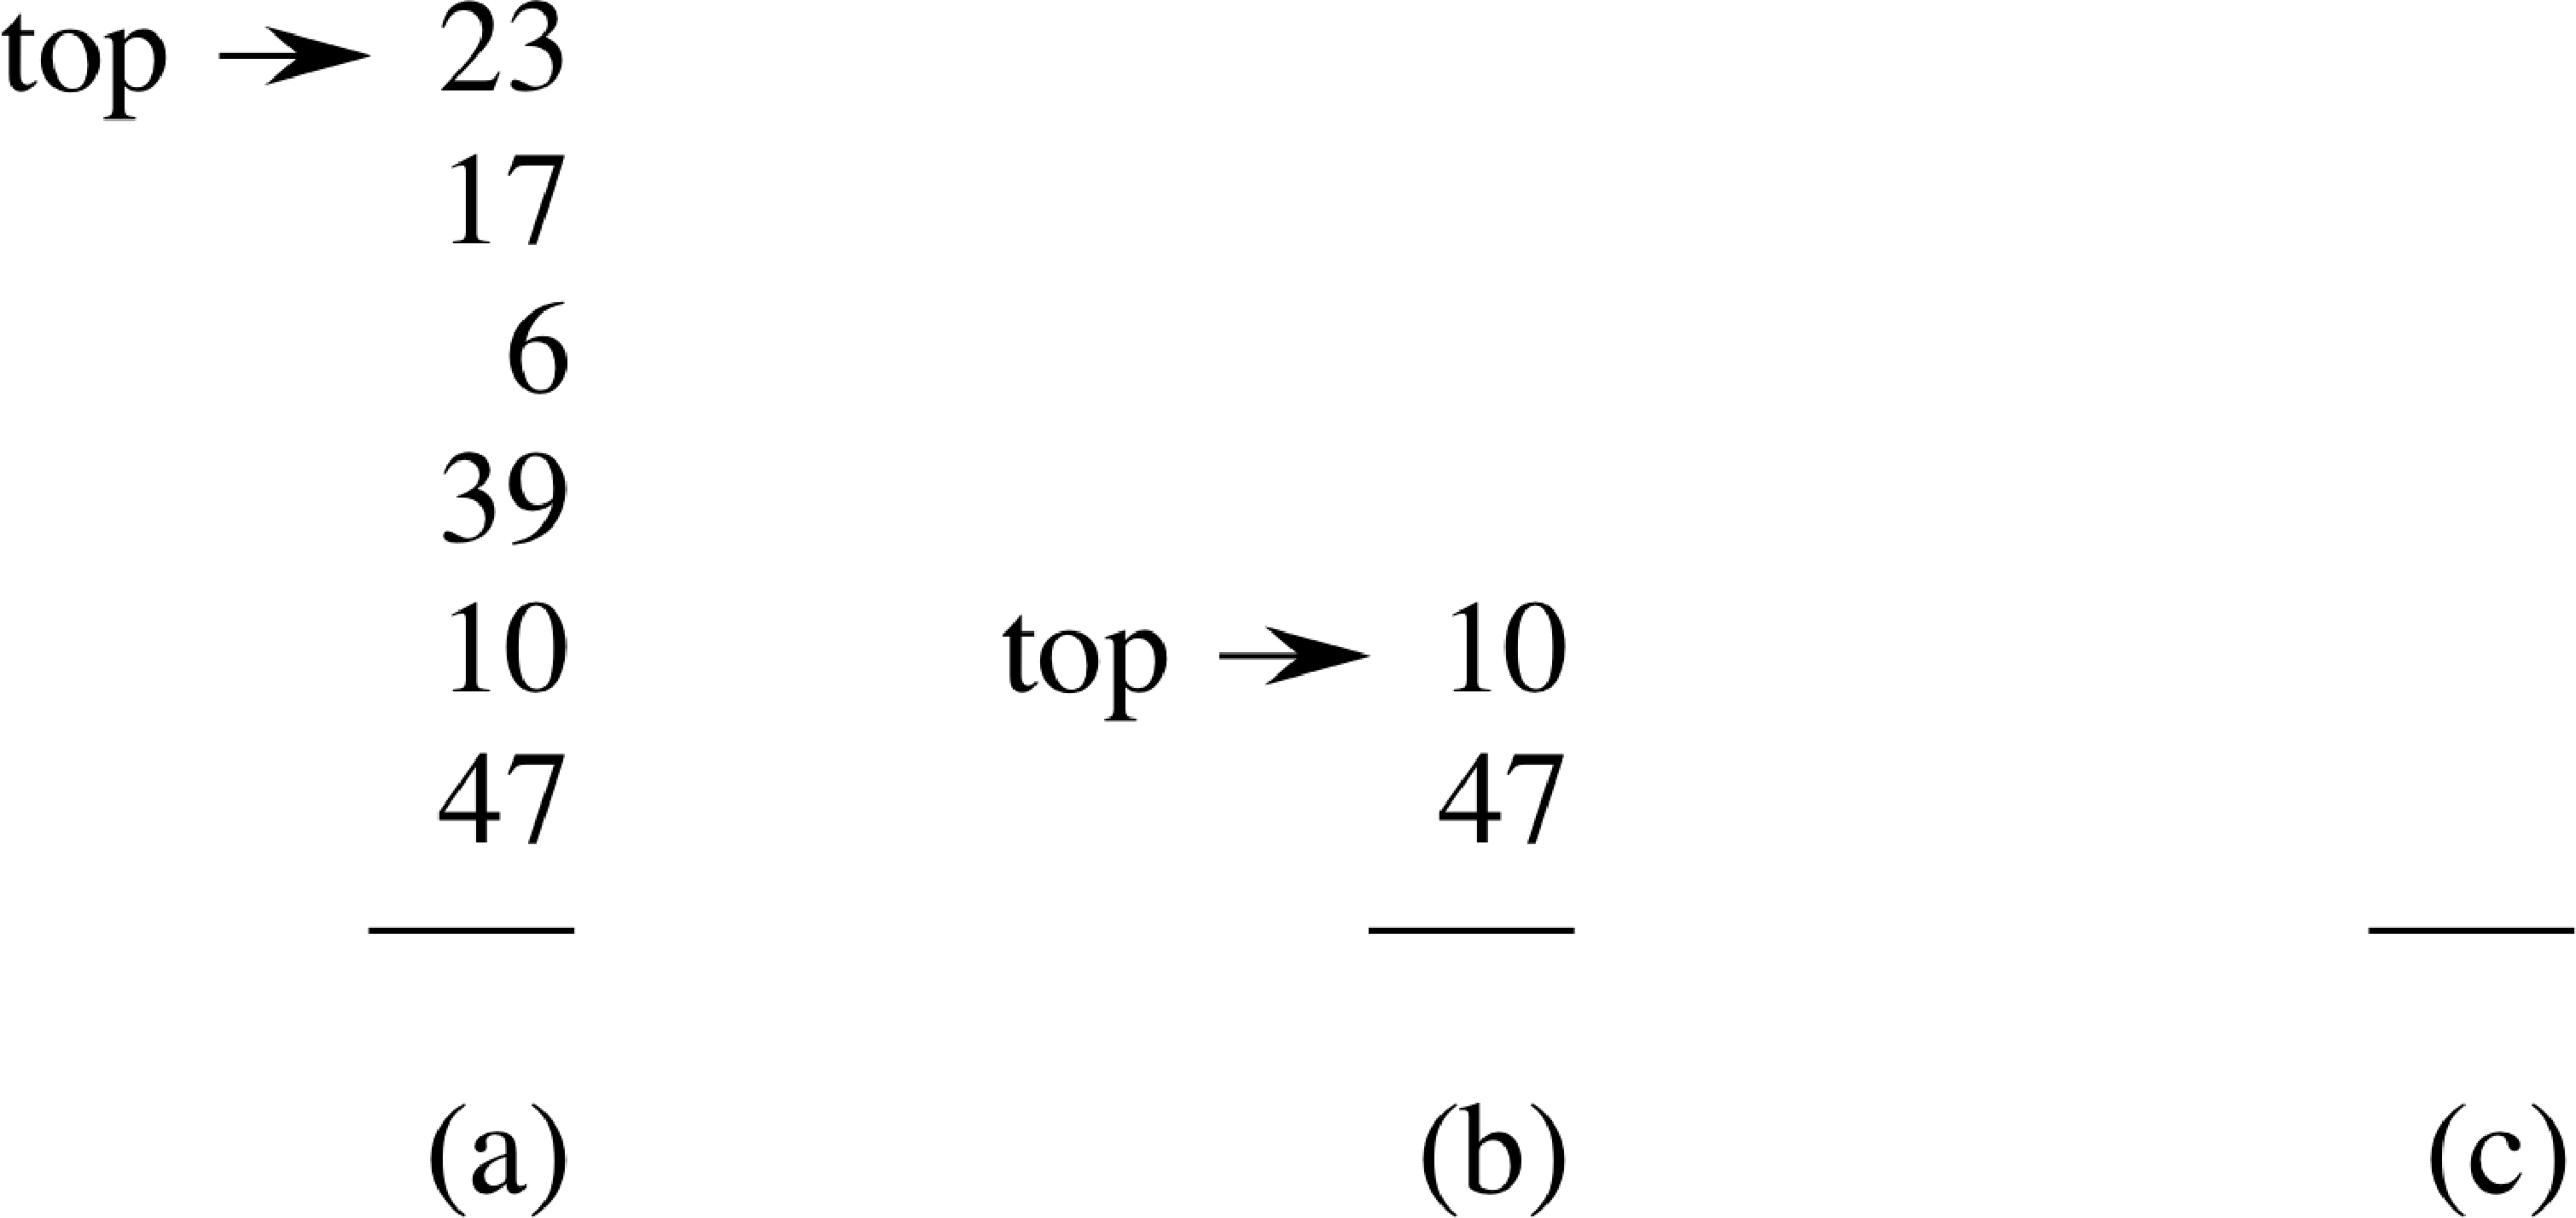
\includegraphics[width=0.7\textwidth]{Fig-17-1.pdf}\\
\mbox{}\hspace{0cm}$\textsc{Multipop}(S,4)$
\hspace{1cm}$\textsc{Multipop}(S,7)$

\end{frame}

\sect{Running time of \textsc{Multipop}:}
\bi
\ii Linear in \# of \textsc{Pop} operations.
\ii Let each \textsc{Push/Pop} cost 1.
\ii \# iterations of \textbf{while} loop is $\min(s,k)$
\bi\ii where $s=$ \# of objects in stack. \ei
\ii Total cost $=\min(s,k)$
\ei




\end{frame}

\sect{Worst-case analysis without amortization}
\bi
\ii Sequence of $n$ \textsc{Push}, \textsc{Pop}, and \textsc{Multipop}
operations.
\ii May have up to $n$ \textsc{Push} operations.
\ii So worst-case there are $n$ items on the stack.
\ii Therefore, worst-case cost of a \textsc{Multipop} operation is $O(n)$.
\ii Have $n$ operations, each of which could be \textsc{Multipop}.
\ii Therefore, worst-case cost of sequence of $n$ operations is
$O(n^2)$.
\ei
\end{frame}

\sect{Something wrong with worst-case analysis}
\bi
\ii There's clearly something wrong with this analysis.
\ii What is actual worst-case number of \textsc{Push}s and \textsc{Pop}s
as a function of $n$?
\ii But how can we get a more accurate worst-case analysis?
\ii We need to consider how the operations interact with each other.
\ii We need to keep an account of how much time is spent in each one,
because that affects the time spent in the others.
\ei


\end{frame}

\sect{Aggregate analysis}
\bi
\ii {\bf Observations}
\bi
\ii Each object can be popped only once per time that it's pushed.
\ii Have $\leq n$ \textsc{Push}s, therefore $\leq n$ \textsc{Pop}s,
including those in \textsc{Multipop}.
\ii Therefore, total cost $=O(n)$.
\ii Average over $n$ operations is $=O(1)$ per operation on average,
including those in \textsc{Multipop}.
\ei
\ii This is called {\bf aggregate analysis}.
\bi
\ii No probability involved.
\ii Showed worst-case $O(n)$ for entire sequence.
\ii Therefore, $O(1)$ per operation on average.
\ei\ei

\end{frame}

\sect{Binary counter}
\begin{multicols}{2}
  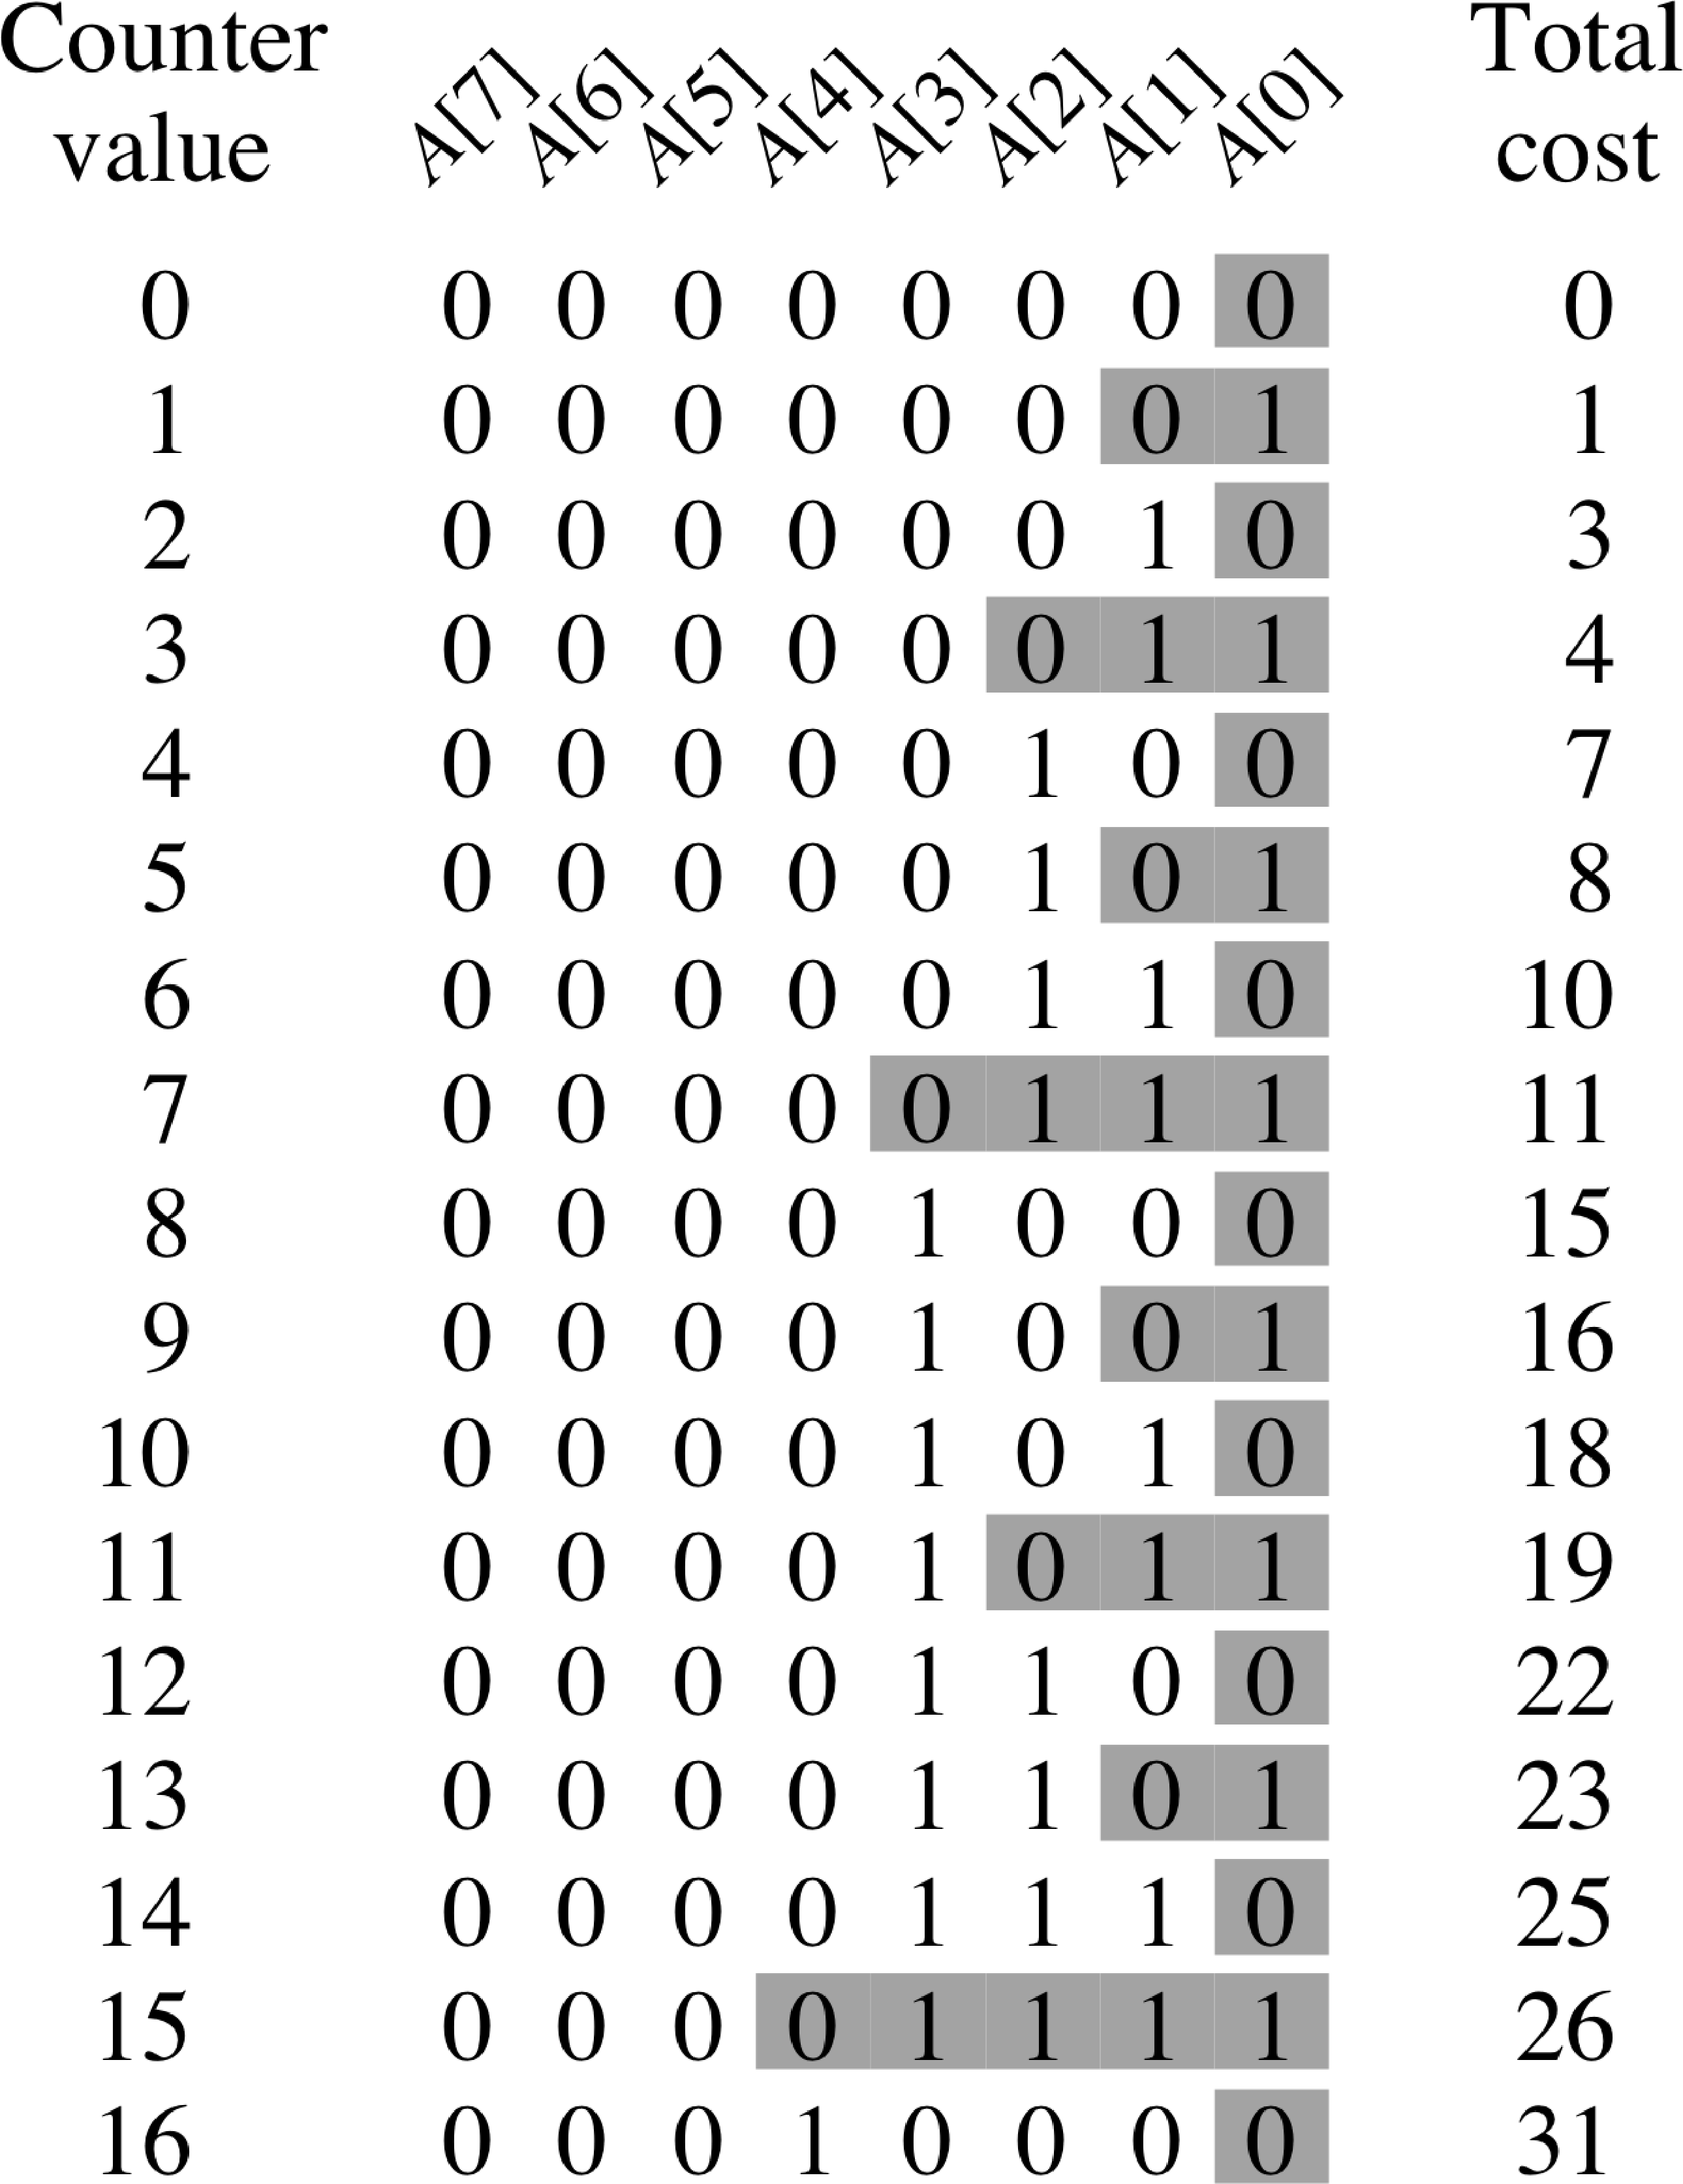
\includegraphics[scale=0.125]{Fig-17-2.pdf}
\columnbreak
  \bi
  \ii Bits that flip upon increment shaded.
  \ii Total cost of flipping bits at right.
  \ii Total cost always less than twice number of increments.
  \ei
\end{multicols}

\end{frame}

\sect{Binary counter}
%\begin{multicols}{2}
\bi
\ii $k$-bit binary counter $A[0..k-1]$ of bits.
\ii $A[0]$ is the least significant bit.
\ii Counts upward from 0.
\ii Value of counter is \[\sum_{i=0}^{k-1} A[i]\cdot 2^i\]
\ii Initially counter is 0, so $A[0..k-1] = 0$.
\ii To increment, add 1 (mod $2^k$):
\ei
%\columnbreak
\begin{codebox}
  \Procname{$\proc{Increment}(A,k)$}
  \li $i\gets 0$
  \li \While $i<k$ and $A[i] \isequal 1$ \Do
  \li $A[i]\gets 0$ \RComment reset to 0
  \li $i\gets i+1$  \End
  \li \If $i < k$ \Do
  \li $A[i] \gets 1$ \End \RComment set to 1
\end{codebox}
%\end{multicols}
\end{frame}

\sect{Worst case analysis of binary counter}
\bi
\ii Each call could flip $k$ bits.
\ii $n$ increments is $O(nk)$.
\ei

\end{frame}

\sect{Aggregate analysis of binary counter}
\bi
\ii Not every bit flips every time.
\ei
\begin{tabular}{ccc}
  bit & flips how often & times in $n$ \textsc{Increment}s \\\hline
  0 & every time & $n$\\
  1 & 1/2 the time & \flr{n/2} \\
  2 & 1/4 the time & \flr{n/4}\\
  & $\vdots$ & \\
  $i$ & $1/2^i$ the time & \flr{n/2^i}\\
  & $\vdots$ & \\
  $i\geq k$ & never & 0 \\
  \end{tabular}


\end{frame}

\sect{Total number of flips}
\begin{align*}
  \sum_{i=0}^{k-1}\flr{n/2^i}
  &< n\sum_{i=0}^{\infty}{1/2^i}\\
  &= n\left(\frac{1}{1-1/2}\right)\\
  &= 2n
\end{align*}

\bi
\ii $n$ \textsc{Increment}s costs $O(n)$.
\ii Average cost per operation $O(1)$.
\ei


\end{frame}

\sect{Accounting Method and Potential Method}

\bi
\ii Aggregate method works when we can add up all operations.
\ii More complex operations need a more sophisticated method.
\ii Two approaches:
\ii \textbf{Accounting method:}
\bi
\ii  assign charges to each operation
\ii some operations charged more than they cost
\ii others, charged less, can use accrued credit
\ei
\ii \textbf{Potential method:}
\bi
\ii prepaid work is ``potential energy''
\ii energy is assigned to data structures as a whole
\ii some operations increase potential energy
\ii some operations can release potential energy to reduce costs
\ii most flexible of the amortized analysis methods
\ei
\ei


\end{frame}

\sect{Accounting method}
\bi
\ii \textbf{Amortized cost} = amount we charge
\ii Amortized cost must always be $\geq$ actual cost
\ii When amortized cost $>$ actual cost, store the difference \textit{on
  specific objects} in the data structure as \textbf{credit}.
\ii When we have credit, we have accounted for expenses not yet accrued
\ii Use credit later to pay for operations whose actual cost $>$
amortized cost.
\ii Differs from aggregate analysis:
\bi
\ii In the accounting method, different operations can have different
costs.
\ii In aggregate analysis, all operations have the same cost.
\ei
\ii Credit must never go negative.
\bi
\ii Otherwise we have a sequence of operations for which amortized
cost is not an upper bound on actual cost.
\ii Amortized cost would tell us nothing.
\ei
\ei


\end{frame}

\sect{Accounting method costs}

\begin{align*}
  c_i &= \mbox{actual cost of $i$th operation}\\
  \hat{c_i} &= \mbox{amortized cost of $i$th operation}
\end{align*}
Require, for {\em all} sequences of $n$ operations:
\begin{align*}
  \sum_{i=1}^{n}\hat{c_i} &\geq   \sum_{i=1}^{n}{c_i} 
\end{align*}
Total credit stored
\begin{align*}
  \sum_{i=1}^{n}\hat{c_i} -   \sum_{i=1}^{n}{c_i} 
\end{align*}
must never be negative.


\end{frame}

\sect{Accounting method amortized analysis of stack operations}
\vfill

\begin{tabular}{lcc}
  operation & actual cost & amortized cost\\\hline
  \textsc{Push} & 1 & 2 \\
  \textsc{Pop} & 1 & 0 \\
  \textsc{Multipop} & min$(k,s)$ & 0
\end{tabular}
\vfill
{\bf Intuition:}
\bi
\ii When pushing an object, pay \$2
\ii \$1 pays for the \textsc{Push}
\ii \$1 is prepayment for it being popped by \textsc{Pop} or
\textsc{Multipop}
\ii Since each object has \$1 credit, the credit can never go
negative.
\ii Total amortized cost, $O(n)$, is an upper bound on total cost.
\ii Worst cast amortized cost is $2n=O(n)$.
\ei

\vfill

\end{frame}

\sect{Accounting method amortized analysis of binary counter}

\bi
\ii Charge \$0 to set a bit to 0
\ii Charge \$2 to set a bit to 1
\bi
\ii \$1 pays for setting the bit to 1
\ii \$1 prepayment for setting it back to 0
\ii Have \$1 credit for every 1 in the counter
\ii Therefore credit $\geq 0$
\ei

\ii Amortized cost of \textsc{Increment}:
\bi
\ii Cost of resetting bits to 0 is paid by credit.
\ii At most 1 bit is set to 1.
\ii Amortized cost is always $\leq 2$.
\ii For $n$ operations amortized cost is $O(n)$.
\ei
\ei

\end{frame}

\sect{The Potential Method}
\bi
\ii Like the accounting method, but think of the credit
as the \textsl{potential} stored with the entire data structure.
\ii Accounting method stores credit with specific objects.
\ii Potential method stores potential in the data structure as a
whole.
\ii Can release potential to pay for future operations.
\ii Most flexible of the amortized analysis methods.
\ei

\end{frame}

\sect{Potential function}
\begin{align*}
  D_i &= \mbox{data structure after the $i$th operation}\\
  D_0 &= \mbox{initial data structure}\\
  c_i &= \mbox{actual cost of $i$th operation}\\
  \hat{c_i} &= \mbox{amortized cost of the $i$th operation}
\end{align*}

\textbf{Potential function:} $\Phi:D_k\rightarrow \mathbb{R}$

$\Phi(D_i)$ is the \textit{potential} associated with the data
structure $D_i$.

\begin{align*}
  \hat{c_i} &= c_i + \Phi(D_i) - \Phi(D_{i-1})\\
  &= c_i + \Delta\Phi(D_i)
\end{align*}

The amortized cost is the \textit{increase in potential} due to the
$i$th operation.

\end{frame}

\sect{Total amortized cost}

\begin{align*}
   \sum_{i=1}^{n} \hat{c_i} 
  &= \sum_{i=1}^{n} (c_i + \Phi(D_i) - \Phi(D_{i-1}))\\
  &= \sum_{i=1}^{n} c_i + \Phi(D_n) - \Phi(D_0)
\end{align*}

\bi
\ii If we require that $\Phi(D_i)\geq \Phi(D_0)$ for all $i$, then the
amortized cost is always an upper bound on the actual cost.
\ii In practice:
\begin{align*}
  \Phi(D_0) &= 0\\
  \Phi(D_i) &\geq 0 &\mbox{for all $i$}
\end{align*}
\ei

\end{frame}

\sect{Amortized analysis of stack operations using the potential
  method}
\begin{align*}
  \Phi &= \mbox{\# of objects in the stack}\\
  &= \mbox{\# of \$1 bills in the accounting method}\\
\Phi(D_0) &= 0
\end{align*}
\vfill

Since \# of objects in stack is always $\geq 0$,
\begin{align*}
  \Phi(D_i) &\geq 0 = \Phi(D_0) &\mbox{for all $i$}
\end{align*}

Let $s =$ \# objects intially
\[
\begin{array}{lccc}
\mbox{operation} & \mbox{actual cost} & \Delta\Phi & \mbox{amortized cost} \\\hline
  \textsc{Push} & 1 & (s+1)-s = 1 & 1+1=2\\
  \textsc{Pop} & 1 & (s-1)-s = -1 & 1-1=0\\
  \textsc{Multipop} & k'=\min(k,s) & (s-k')-s = -k' & k'-k' = 0\\
\end{array}
\]
\vfill

Therefore the amortized cost of a sequence of $n$ operations is $O(n)$.


\vfill

\end{frame}

\sect{Amortized analysis of binary counter: potential method}
\small
\bi
\ii
$\Phi = b_i = $ \# of 1's after $i$th \textsc{Increment}
\ii
Suppose $i$th operation resets $t_i$ bits to 0.

\ii
$c_i \leq t_i + 1$, since it resets $t_i$ bits and sets $\leq 1$ bit
to 1.


\ii If $b_i=0$, the $i$th operation reset all $k$ bits and didn't set
one, so
\[ b_{i-1} = t_i = k \Rightarrow b_i = b_{i-1} - t_i = 0\]
\ii If $b_i > 0$ the $i$th operation reset $t_i$ bits, set one, so
\[ b_i = b_{i-1} - t_i + 1\]
\ii Either way
\[ b_i \leq b_{i-1} -t_i + 1\]
\ii Therefore
\begin{align*}
  \Delta\Phi(D_i) &\leq (b_{i-1} - t_i + 1) - b_{i-1}
  = 1-t_i\\
  \hat{c_i} &= c_i + \Delta\Phi(D_i)
  \leq (t_i + 1) + (1-t_i) = 2
\end{align*}

\ii If counter starts at 0, $\Phi(D_0) = 0$.

\ii Therefore, amortized cost of $n$ operations is $O(n)$.

\ii Method works even if counter does not start at 0.
\ei



\end{frame}

\sect{Dynamic Tables}
\bi
\ii Nice application of amortized analysis.
\ii Suppose you have a table, maybe a hash table, maybe a heap.
\ii Details of table organization not important.
\ii We will assume
insertion and deletion take $O(1)$.
\ii You don't know in advance how many items will be stored in it.
\ii When it fills, you must reallocate a larger table and copy all the
items into the new table.
\ii When it gets sufficiently small, you \textit{might} want to
reallocate with a smaller size.
\ii How can you do this so it doesn't mess up the efficiency of your
table?
\ii Does it turn $O(1)$ (hash) or $O(\lg n)$ (heap) into $O(n)$, since
in worst case we have to copy all $n$ elements into new array?
\ei

\end{frame}

\sect{Dynamic Table Goals}
\begin{enumerate}
\ii $O(1)$ amortized time per operation.
\ii Unused space always $\leq$ constant fraction of allocated space.
\end{enumerate}
\bi
\ii \textbf{Load factor} $\alpha=\id{num}/\id{size}$ where $\id{num}
=$ \# items stored, $\id{size} =$ allocated size.
\ii Never allow $\alpha > 1$
\ii Keep $\alpha >$ constant fraction (goal 2).
\ei


\end{frame}

\sect{Table expansion}
\small
\bi
\ii First we consider only expansion.
\ii When table becomes full, double its size and reinsert all existing
items.
\ii Each time we actually insert an item, it's an \textbf{elementary
  insertion}.
\ei
\begin{codebox}
  \Procname{$\proc{Table-Insert}(T,x)$}
  \li \If $\attrib{T}{size} \isequal 0$ \Do \RComment empty?
  \li allocate $\attrib{T}{table}$ with 1 slot
  \li $\attrib{T}{size} \gets 1$ \End
  \li \If $\attrib{T}{num}\isequal\attrib{T}{size}$ \Do  \RComment expand?
  \li allocate $\id{new-table}$ with $2\cdot\attrib{T}{size}$ slots
  \li insert all items in $\attrib{T}{table}$ into $\id{new-table}$
  \li free $\attrib{T}{table}$
  \li $\attrib{T}{table}\gets \id{new-table}$
  \li $\attrib{T}{size}\gets 2\cdot\attrib{T}{size}$ \End
  \li insert $x$ into $\attrib{T}{table}$
  \li $\attrib{T}{num} \gets \attrib{T}{num} + 1$
  \end{codebox}
  
  
\end{frame}

\sect{Running time}
\bi
\ii Charge 1 per elementary insertion.
\ii Count only elementary insertions.
\bi \ii All other costs are constant per cell.\ei
\ii $c_i = $ actual cost of $i$th operation
\ii If not full, $c_i = 1$
\ii If full, insert $i-1$ items plus one more, $c_i=i$.
\ii $n$ operations, worst case:
\ei
\begin{align*}
c_i&=O(n)\\
\mbox{$n$ operations} &= O(n^2)
\end{align*}

\end{frame}

\sect{Aggregate analysis}

  \bi
  \ii Of course, we don't \textit{always} expand:
  \ei
\[
c_i = \left\{\begin{array}{ll}
i & \mbox{if $i-1$ is exact power of 2.}\\
  1 & \mbox{otherwise.}\end{array}\right.
\]
\begin{align*}
  \mbox{Total cost} &= \sum_{i=1}^{n} c_i\\
  &\leq n + \sum_{j=0}^{\flr{\lg n}} 2^j\\
  &= n + \frac{2^{\flr{\lg n} + 1} -1}{2-1}\\
  &< n + 2n\\
  &= 3n
\end{align*}

\bi
\ii Aggregate analysis: the amortized cost per operation is 3.
\ei


\end{frame}

\sect{Accounting method}

\bi
\ii Charge \$3 per elementary insertion of $x$:
\bi
\ii \$1 pays for $x$'s insertion.
\ii \$1 pays for $x$'s move in the future.
\ii \$1 pays for some other item to be moved.
\ei

\ii Suppose we've just expanded, $\id{size} = m$.
\ii $\id{size} = 2m$ after next expansion.

\ii Assume that the expansion used up all the credit, so that there's
no credit stored after the expansion.
\ii Will expand again after another $m$ insertions.

\ii Each insertion will put \$1 on one of the $m$ items that were in
the table just after expansion, and will put \$1 on the item inserted.
\ii Have \$2$m$ of credit by next expansion, when there are $2m$ items
to move.
\ii Just enough to pay for expansion, with no credit left over!
\ii Credit always $\geq 0$.
\ei

\end{frame}

\sect{Potential method}

\[
\Phi(T) = 2\cdot\attrib{T}{num}-\attrib{T}{size}
\]
\bi
\ii Initially, $\id{num} = \id{size} = 0$.
\[\Phi = 0\]
\ii Just after expansion, $\id{size} = 2\cdot\id{num}$
\[\Phi = 0\]
\ii Just before expansion, $\id{size} = \id{num}$
\[\Phi = \id{num}\]
we have enough potential to pay for moving all items.
\ii Need $\Phi\geq 0$ always.
\[
\begin{array}{cccccc}
  \id{size} & \geq & \id{num} & \geq & \id{size}/2 & \Rightarrow \\
  &       & 2\cdot\id{num} & \geq & \id{size} & \Rightarrow\\
  &       & \Phi & \geq & 0
\end{array}
\]

\ei

\end{frame}

\sect{Amortized cost of $i$th operation}

\begin{align*}
  \id{num}_i &= \mbox{$\id{num}$ after $i$th operation}\\
  \id{size}_i &= \mbox{$\id{size}$ after $i$th operation}\\
  \Phi_i &= \mbox{$\Phi$ after $i$th operation}
\end{align*}
\bi
\ii If no expansion:
\begin{align*}
  \id{size}_i &= \id{size}_{i-1}\\
  \id{num}_i &= \id{num}_{i-1} + 1\\
  c_i &= 1
\end{align*}
Then we have
\begin{align*}
  \hat{c_i} &= c_i + \Phi_i - \Phi_{i-1}\\
  &= 1 + (2\cdot\id{num}_i - \id{size}_i) - (2\cdot\id{num}_{i-1} -
  \id{size}_{i-1}) \\
  &= 1 + (2\cdot\id{num}_i - \id{size}_i) - (2(\id{num}_{i}-1) -
  \id{size}_{i}) \\
  &= 1 + 2 = 3
\end{align*}

\ei

\end{frame}
\small
\sect{Amortized cost of $i$th operation}
\bi
\ii If expansion:
\begin{align*}
  \id{size}_i &= 2\cdot\id{size}_{i-1}\\
  \id{size}_{i-1} &= \id{num}_{i-1} = \id{num}_{i} -1\\
  c_i &= \id{num}_{i-1} + 1 = \id{num}_{i}
\end{align*}
Then we have
\begin{align*}
  \hat{c_i} &= c_i + \Phi_i - \Phi_{i-1}\\
  &= \id{num}_i + (2\cdot\id{num}_i-\id{size}_i) -
  (2\cdot\id{num}_{i-1}-\id{size}_{i-1})\\
  &= \id{num}_i + (2\cdot\id{num}_i-2(\id{num}_i-1)) -
  (2(\id{num}_{i}-1)-(\id{num}_{i}-1))\\
  &= \id{num}_i + 2 - (\id{num}_i - 1)\\
  &= 3
\end{align*}
\ei
\end{frame}

\sect{}
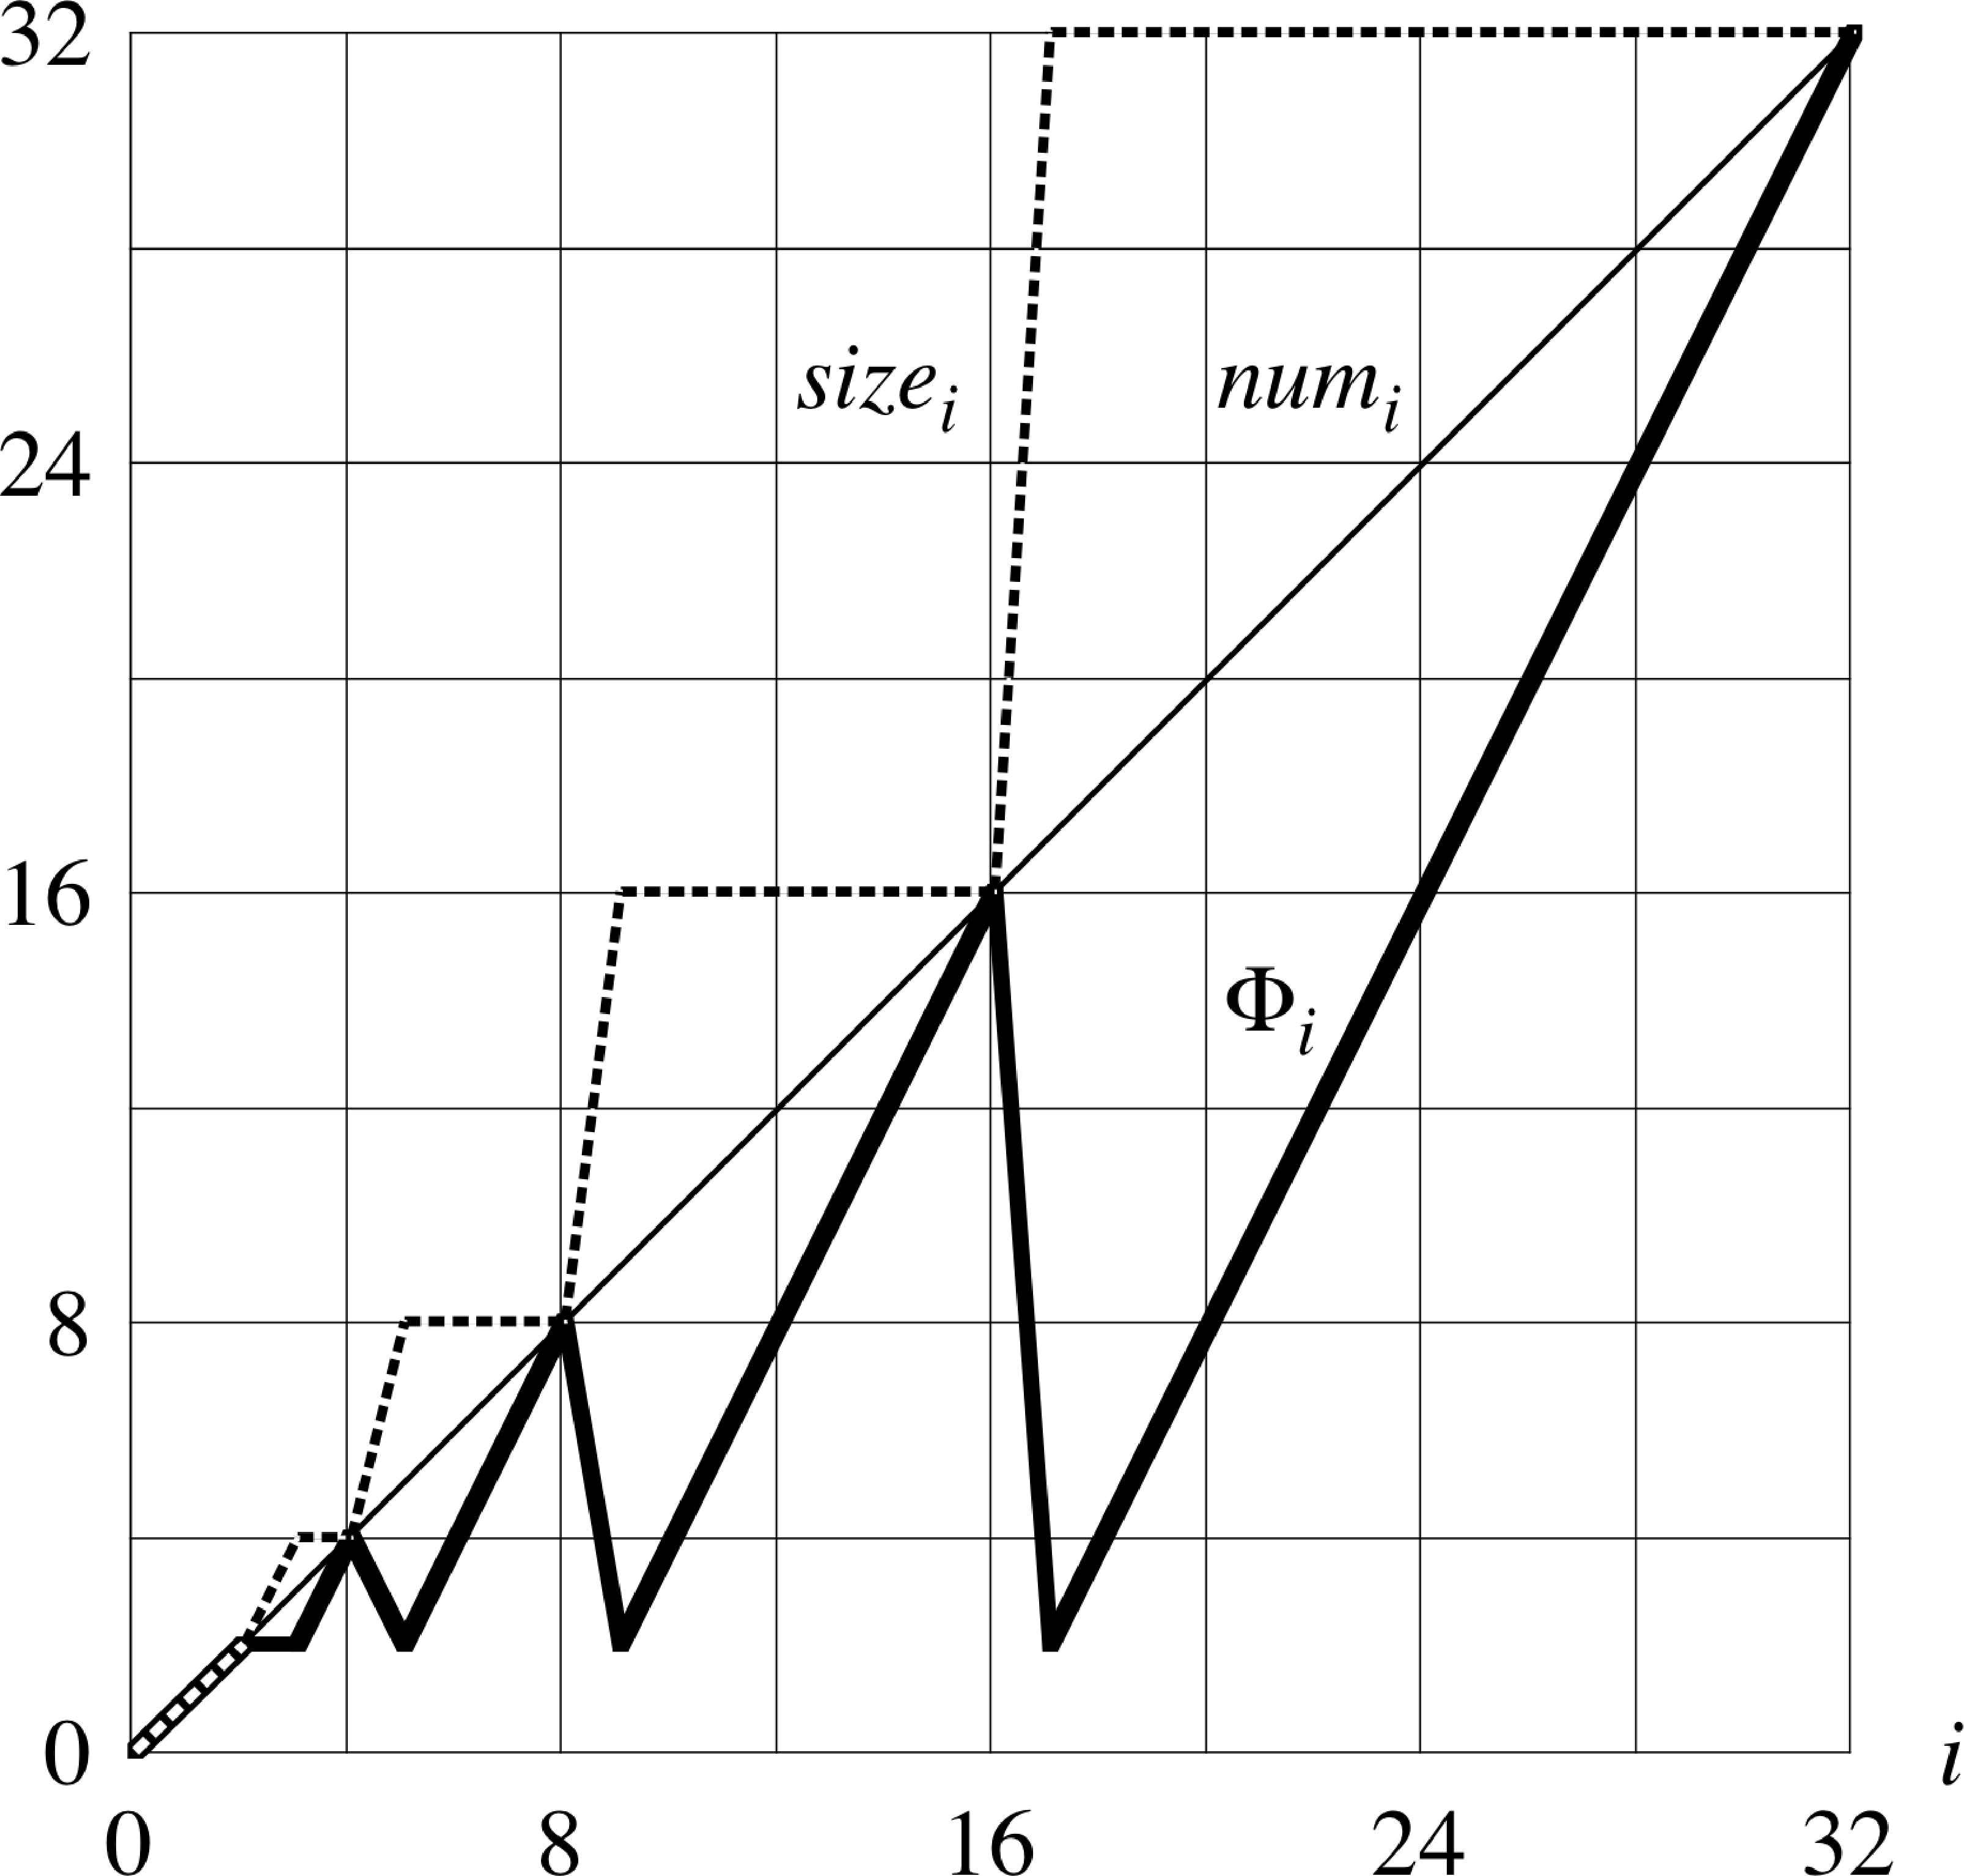
\includegraphics[scale=0.125]{Fig-17-3.pdf}

\bi
\ii As we insert items, the potential builds up until we have enough
to pay for moving all items, when the potential drops back to zero.
\ei

\end{frame}

\sect{Expansion and contraction}

 When $\alpha$ drops too low, contract the table.
\bi
\ii Allocate a new, smaller one.
\ii Copy all items.
\ei
Still want:
\bi
\ii $\alpha$ bounded from below by a constant
\ii amortized cost of $O(1)$
\ei

\end{frame}

\sect{``Obvious strategy''}
\bi
\ii Double size when inserting into a full table ($\alpha = 1$).
\ii Halve size when deletion would make table less than half full
($\alpha < 1/2$).
\ii Then would always have $1/2 \leq \alpha \leq 1$.
\ii Unfortunately, suppose we fill the table, then:

\begin{tabular}{rcl}
insert & $\Rightarrow$ & double\\
two deletes & $\Rightarrow$ & halve\\
two inserts & $\Rightarrow$ & double\\
two deletes & $\Rightarrow$ & halve\\
two inserts & $\Rightarrow$ & double\\&...
\end{tabular}
\ii Not performing enough operations in between expansion and
contraction to pay for the next one.
\ei

\end{frame}

\sect{Simple solution}
\bi
\ii Double when full ($\alpha = 1$).
\ii Halve size when $\alpha = 1/4$.
\ii Immediately after expansion \textit{or} contraction, $\alpha=1/2$.
\ii Always have $1/4\leq\alpha\leq 1$
\ei

\end{frame}

\sect{Intuition}
\bi
\ii Want to make sure we perform enough operations in between
consecutive expansions/contractions to pay for the change in table
size.
\ii Need to delete half of the items before contraction.
\ii Need to double the number of items before expansion.
\ii Either way, the number of operations between expansions and
contractions is at least a constant fraction of the number of items
copied.
\ei

\[
\Phi(T) = \left\{\begin{array}{ll}
2\cdot\attrib{T}{num} - \attrib{T}{size} & \mbox{ if $\alpha \geq
  1/2$}\\
\attrib{T}{size}/2 - \attrib{T}{num} & \mbox{ if $\alpha < 1/2$}
\end{array}\right.
\]

$T$ empty $\Rightarrow \Phi = 0$

$\alpha \geq 1/2 \Rightarrow \id{num} \geq \id{size}/2 \Rightarrow
2\cdot\id{num} \geq \id{size} \Rightarrow \Phi \geq 0$

$\alpha \leq 1/2 \Rightarrow \id{num} < \id{size}/2 \Rightarrow \Phi
\geq 0$

\end{frame}

\sect{}
\[
\Phi(T) = \left\{\begin{array}{ll}
2\cdot\attrib{T}{num} - \attrib{T}{size} & \mbox{ if $\alpha \geq
  1/2$}\\
\attrib{T}{size}/2 - \attrib{T}{num} & \mbox{ if $\alpha < 1/2$}
\end{array}\right.
\]
\centerline{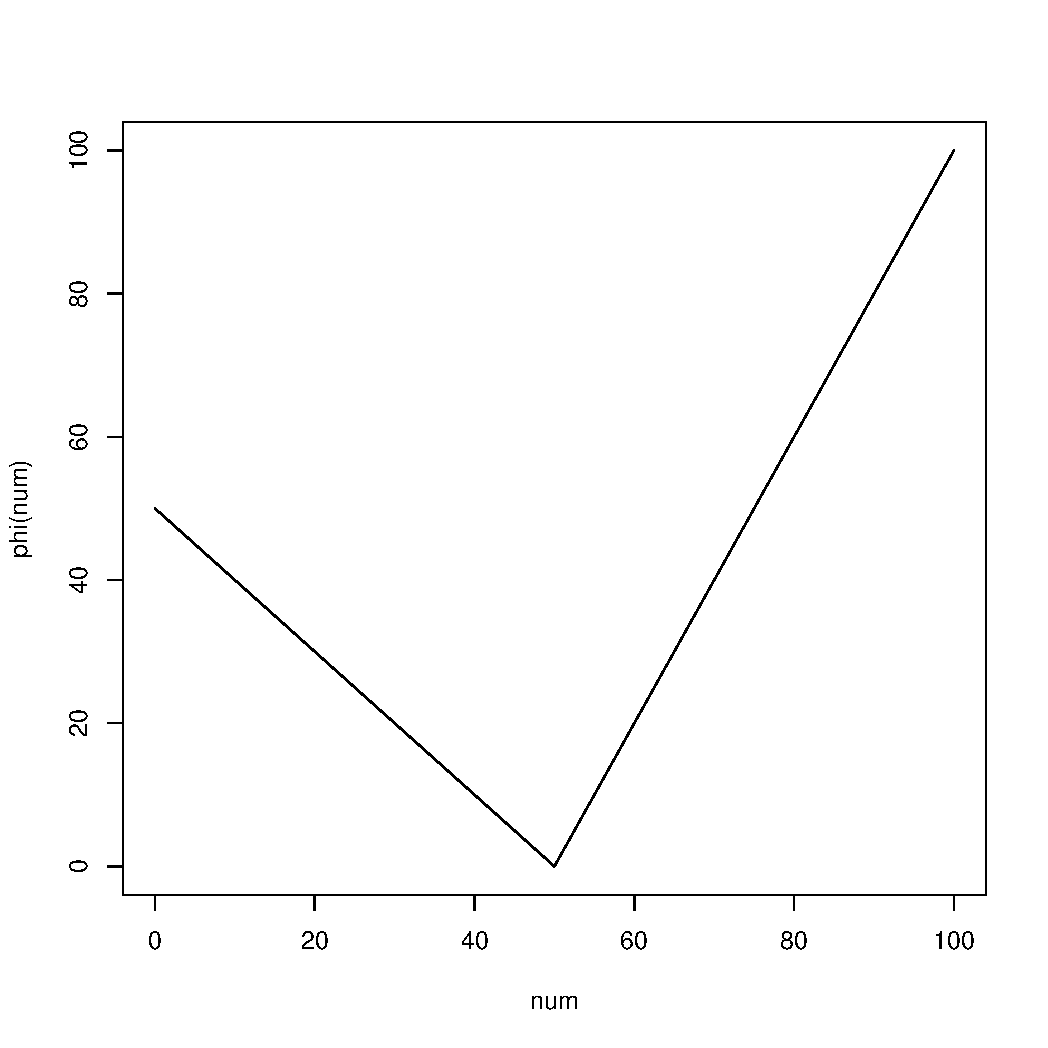
\includegraphics[scale=0.5]{dyntablephi}}

\end{frame}

\sect{Further intuition}
\bi
\ii $\Phi$ measures how far from $\alpha=1/2$ we are.
\ii $\alpha=1/2\Rightarrow \Phi = 2\cdot\id{num} - 2\cdot\id{num} = 0$
\ii $\alpha = 1\Rightarrow\Phi =  2\cdot\id{num} - \id{num} = \id{num}$
\ii $\alpha = 1/4\Rightarrow\Phi =  \id{size}/2 - \id{num} =
4\cdot\id{num}/2-\id{num}=\id{num}$
\ii Therefore, when we double or halve, we have enough potential to
pay for moving all $\id{num}$ items.
\ei
\end{frame}

\sect{Further intuition}
\bi
\ii Potential increases linearly between $\alpha=1/2$ and $\alpha=1$.
\ii Potential increases linearly between $\alpha=1/2$ and
$\alpha=1/4$.
\ii Since $\alpha$ has different distances to go to get to 1 or $1/4$,
starting from $1/2$, rate of increase of $\Phi$ differs.
\ii For $\alpha$ to go from $1/2$ to 1:
\bi
\ii $\id{num}$ increases from $\id{size}/2$ to $\id{size}$
\ii $\Phi$ increases from 0 to $\id{size}$
\ii $\Phi$ needs to increase by 2 for each item inserted.
\ii That's why the coefficient of 2 in the formula for $\Phi$.
\ei
\ii For $\alpha$ to go from $1/2$ to $1/4$:
\bi
\ii $\id{num}$ decreases from $\id{size}/2$ to $\id{size}/4$.
\ii $\Phi$ increases from 0 to $\id{size}/4$
\ii Thus, $\Phi$ needs to increase by 1 for each item deleted.
\ii That's why the coefficient of $-1$ in the formula for $\Phi$.

\ei
\ei




\end{frame}

\sect{Eight cases for calculating amortized costs}
\bi
\ii insert \textit{vs.} delete
\ii $\alpha \geq 1/2$ \textit{vs.} $\alpha < 1/2$
\ii $\id{size}$ changes \textit{vs.} $\id{size}$ doesn't change
\ei

\end{frame}

\sect{Insert, $\alpha\geq 1/2$, with or without expansion}
\bi
\ii Same analysis as before.
\ii $\hat{c_i} = 3$
\ei

\end{frame}

\sect{Insert, $\alpha_{i-1}< 1/2$, no expansion}
\bi
\ii $\alpha_i < 1/2$
\begin{align*}
  \hat{c_i} &= c_i + \Phi_{i} - \Phi_{i-1}\\
  &= 1 + (\id{size}_i/2-\id{num}_i) - (\id{size}_{i-1}/2 -
  \id{num}_{i-1})\\
  &= 1 + (\id{size}_i/2-\id{num}_i) - (\id{size}_{i}/2 -
  (\id{num}_{i}-1))\\
  &= 0
\end{align*}
\ii $\alpha_i \geq 1/2$
\begin{align*}
  \hat{c_i} &= c_i + \Phi_{i} - \Phi_{i-1}\\
  &= 1 + (2\cdot\id{num}_i-\id{size}_i) - (\id{size}_{i-1}/2 -
  \id{num}_{i-1})\\
  &= 1 + (2(\id{num}_{i-1}+1)-\id{size}_{i-1}) - (\id{size}_{i-1}/2 -
  \id{num}_{i-1})\\
  &= 3\cdot\id{num}_{i-1}-\frac{3}{2}\cdot\id{size}_{i-1} + 3\\
  &= 3\cdot\alpha_{i-1}\id{size}_{i-1}-\frac{3}{2}\cdot\id{size}_{i-1} + 3\\
  &< \frac{3}{2}\cdot\id{size}_{i-1}-\frac{3}{2}\cdot\id{size}_{i-1} + 3\\
  &= 3
\end{align*}
\ei

\end{frame}

\sect{Insert, $\alpha<1/2$, expansion}
\bi
\ii Cannot happen.
\ei

\end{frame}

\sect{Insert}

\begin{tabular}{lcc}
expansion  & $\alpha \geq 1/2$ &  $\hat{c_i} = 3$ \\
no expansion & $\alpha \geq 1/2$ &  $\hat{c_i} = 3$ \\
expansion & $\alpha < 1/2$ &  impossible\\
no expansion & $\alpha_{i-1}<1/2, \alpha_{i} < 1/2$ & $\hat{c_i} = 0$\\
no expansion &  $\alpha_{i-1} < 1/2, \alpha_{i}\geq 1/2$  &  $\hat{c_i} = 3$\\
\end{tabular}

\bi
\ii Therefore, in all cases, the amortized cost of insertion is $\leq 3$.
\ei


\end{frame}

\sect{Delete}

\begin{tabular}{lcc}
contraction & $\alpha < 1/2$ &  $\hat{c_i} = 1$ \\
no contraction  & $\alpha < 1/2$ &  $\hat{c_i} = 2$ \\
contraction  & $\alpha \geq 1/2$ &  impossible\\
no contraction & $\alpha_{i-1} \geq 1/2, \alpha_{i} \geq 1/2$ & $\hat{c_i} = -1$\\
no contraction &  $\alpha_{i-1} \geq 1/2, \alpha_{i} < 1/2$  &  $\hat{c_i} = 2$
\end{tabular}

\bi
\ii In all cases the
amortized cost is $\leq 2$.
\ei

\vfill

\end{frame}

\sect{}
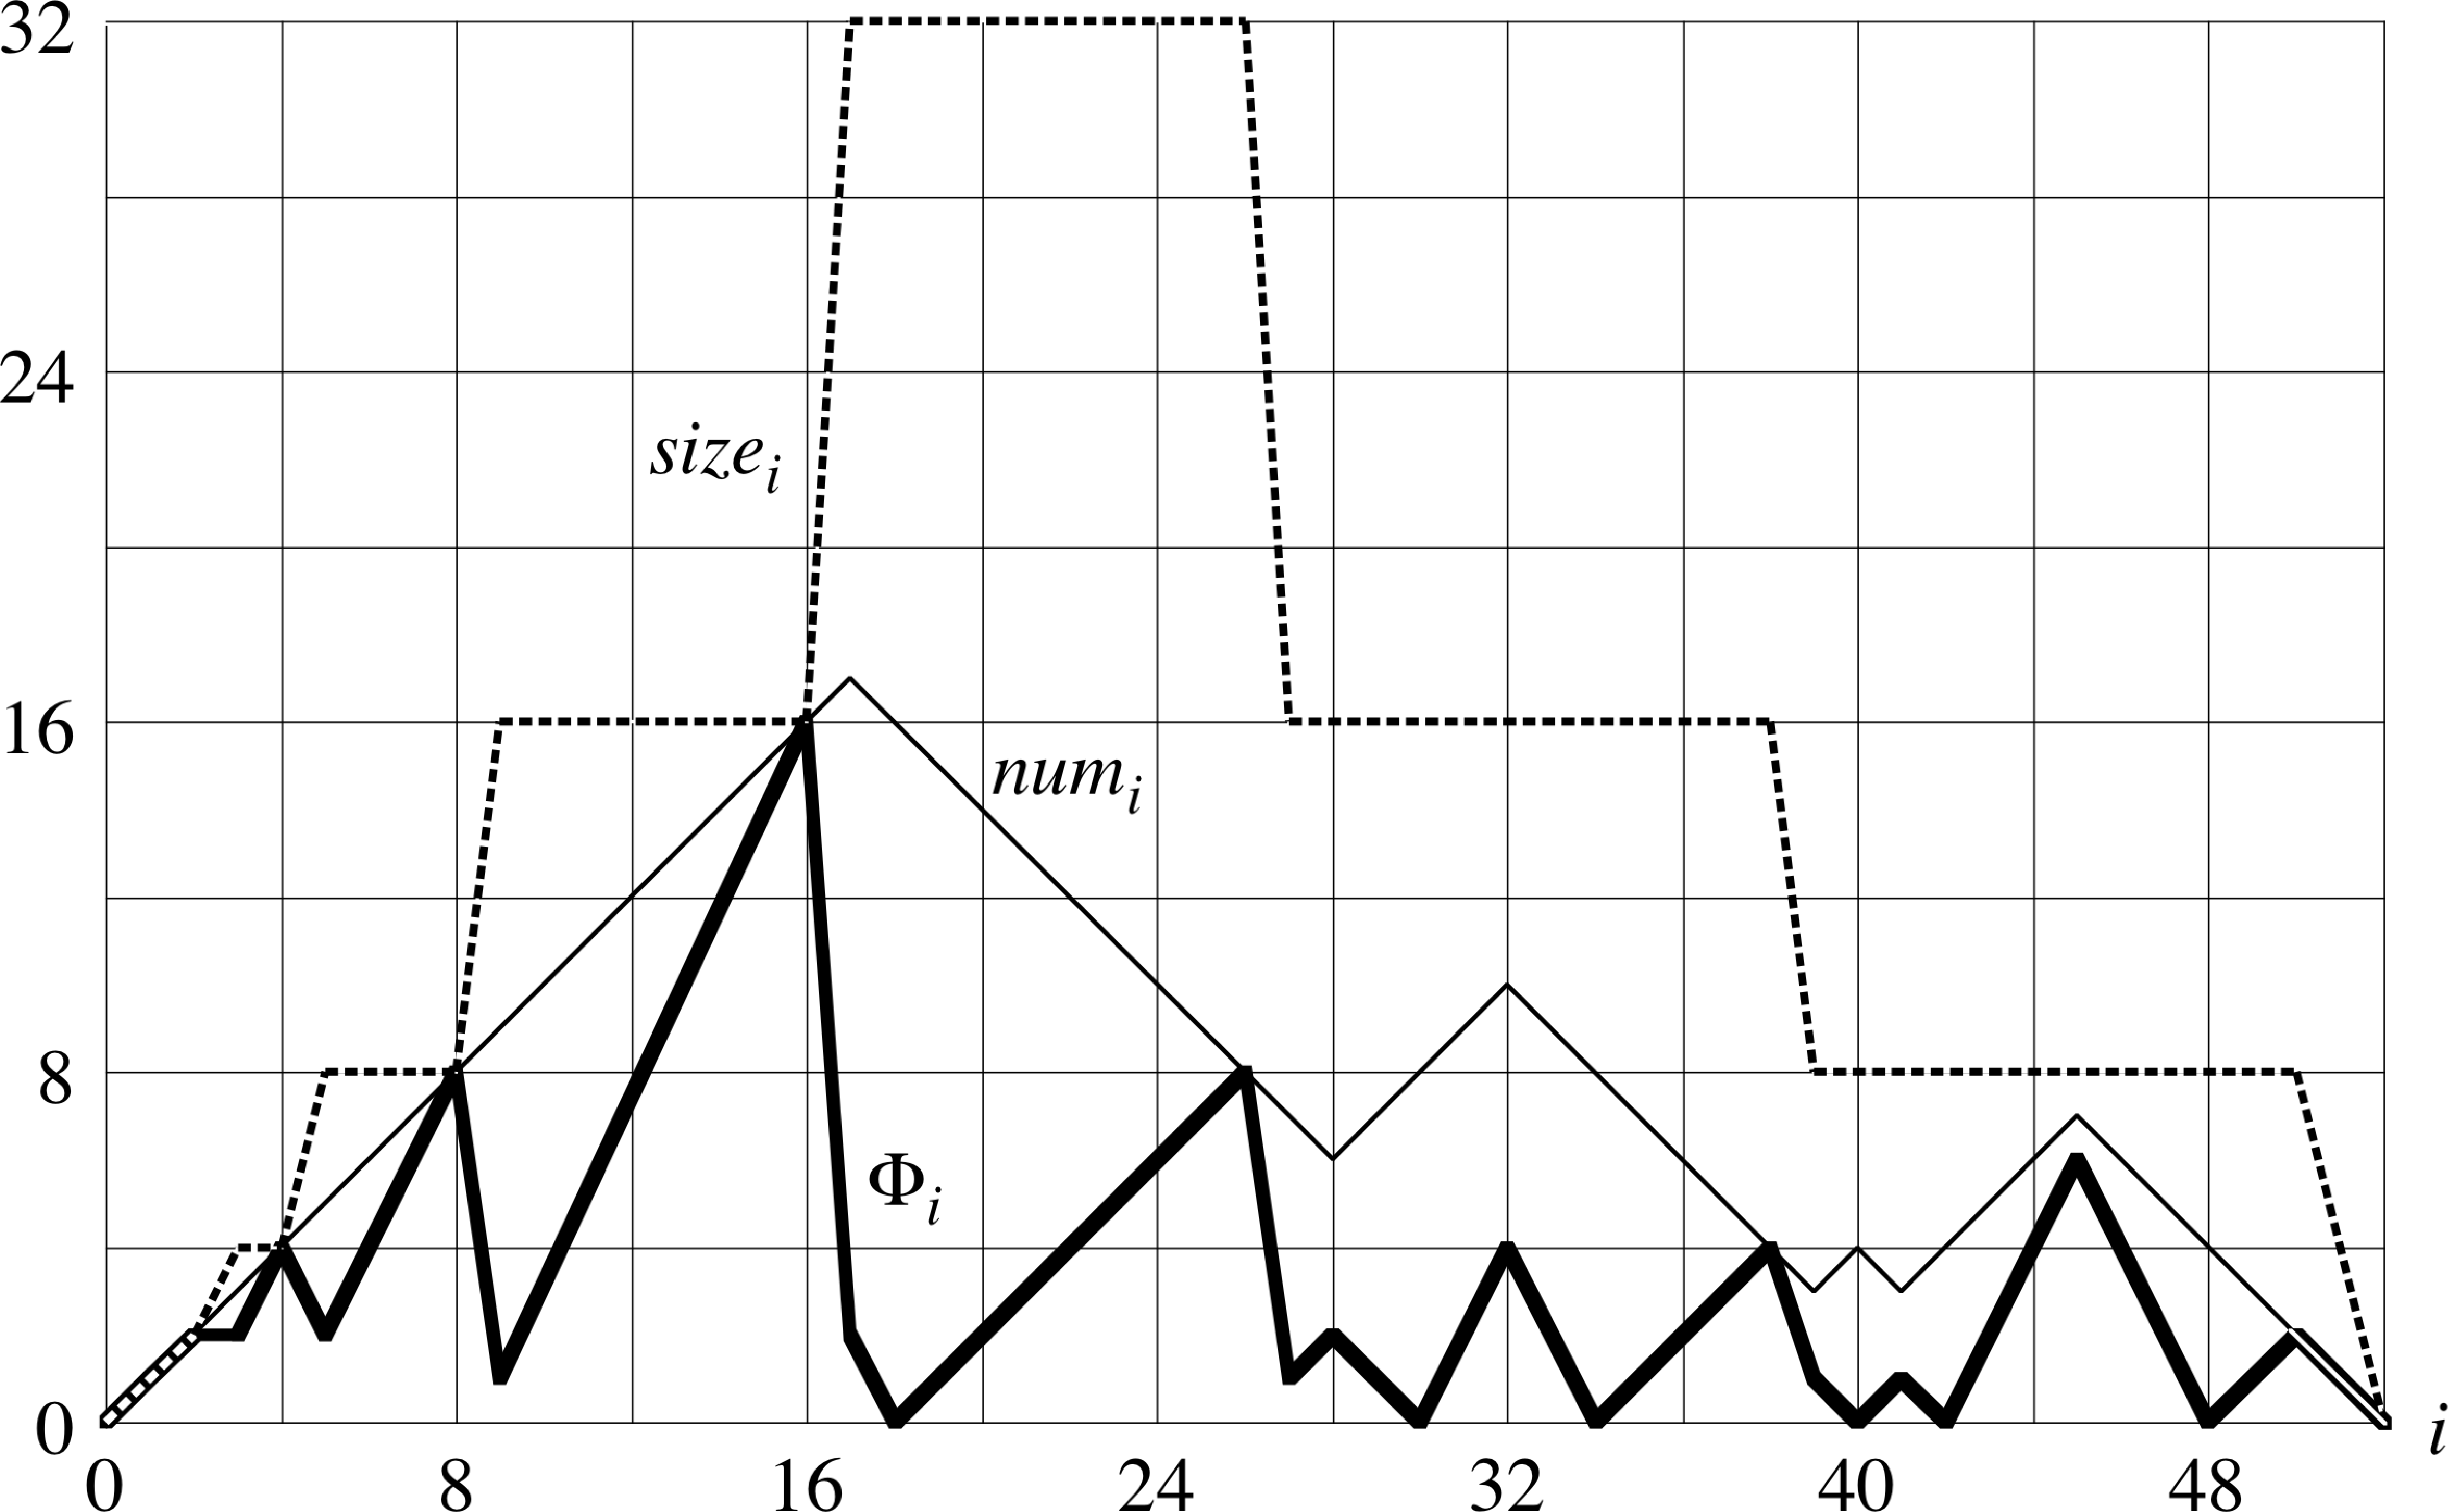
\includegraphics[width=\textwidth]{Fig-17-4.pdf}
\end{frame}

\end{document}
